% Chapter 15 -- Information theory
\chapter{Information theory: bits, entropy, and why the loss is a log}\label{ch:info}

Machine learning's favorite loss function, cross-entropy, is not an
engineering invention --- it is a statement about information. This
chapter builds the short chain from ``how surprised should you be'' to
the softmax loss you have already trained with in chapters 13 and 14.
You will learn what a bit actually measures, why entropy is a lower
bound on any code, why KL divergence is asymmetric, and why minimizing
cross-entropy is maximum likelihood estimation. After this chapter you
can compute entropies and divergences by hand, read a Huffman code's
lengths as approximate $-\log_2 p$, and explain what the CE number in a
training log means --- not just that it went down.

\section{Surprise and information}\label{sec:info-surprise}

An event that happens every time carries no news; an event that almost
never happens carries a lot. We want a measure of ``news'' with three
sane properties: certain events measure zero, rarer events measure
more, and two independent events add. Exactly one family of functions
satisfies all three.

\begin{definition}[Surprise]\label{def:surprise}
The \emph{surprise}\index{surprise} (self-information) of an outcome
$x$ with $\Pr[x]=p$ is
\[
  s(x) \;=\; -\log_2 p \quad\text{bits}.
\]
\end{definition}

Check the three properties: $p=1$ gives $s=0$; smaller $p$ gives larger
$s$; and $\Pr[A\cap B]=\Pr[A]\Pr[B]$ for independent $A,B$ gives
$s(A\cap B)=s(A)+s(B)$ --- the logarithm is doing all the work, and it
is why every quantity in this chapter is a log.

A single flip of a fair coin carries $-\log_2\tfrac12=1$ bit. Rolling a
specific face of a fair die carries $-\log_2\tfrac16\approx 2.585$
bits. A ``bit''\index{bit} is not a digit on a wire --- it is a unit of
surprise: how many fair-coin questions it takes to pin down the
outcome.

\begin{exercise}[easy]
How many bits of surprise does drawing the ace of spades from a shuffled
52-card deck carry? The event ``any ace''?
\end{exercise}

\begin{solution}
$-\log_2\tfrac1{52}=\log_2 52\approx 5.70$ bits;
$-\log_2\tfrac4{52}=\log_2 13\approx 3.70$ bits.
\end{solution}

\section{Entropy and its properties}\label{sec:info-entropy}

Surprise is per-outcome; entropy is the whole distribution's expected
surprise.

\begin{definition}[Entropy]\label{def:entropy}
For a discrete random variable $X$ with pmf $p$, the
\emph{entropy}\index{entropy} is
\[
  H(X) \;=\; \mathbb E[s(X)] \;=\; -\sum_x p(x)\log_2 p(x)
  \quad\text{bits},
\]
with $0\log 0 := 0$ (justified: $p\log p\to 0$ as $p\to0^+$).
\end{definition}

Two facts worth keeping. $H(X)\ge 0$ always, since each
$-p\log_2 p\ge0$. And over $k$ outcomes, $H(X)\le\log_2 k$, with
equality exactly for the uniform distribution --- maximum surprise is
maximum uncertainty (chapter 12's variance played the same role). For a
coin, $h(p)=-p\log_2 p-(1-p)\log_2(1-p)$ is the curve in
Figure~\ref{fig:bernh}: peaked at $p=\tfrac12$, dropping to zero as the
coin gets predictable.

\begin{example}[Entropy of coins and dice]\label{ex:coinentropy}
\textbf{Strategy.} Apply Definition~\ref{def:entropy} directly, then
verify by simulation.

\textbf{Solution.}
A fair coin: $h(\tfrac12)= -\tfrac12\log_2\tfrac12
-\tfrac12\log_2\tfrac12 = 1$ bit. A coin with $p=0.9$:
$h(0.9)=-0.9\log_2 0.9 - 0.1\log_2 0.1 = 0.469$ bits --- biasing the
coin to 90\% threw away more than half the information per flip. A coin
with $p=0.99$: $h=0.081$ bits --- almost nothing left. A fair die:
$H=\log_2 6 = 2.585$ bits. These are exactly the numbers the listing
prints from the formula.

\begin{lstlisting}[caption={\ttfamily code/ch15\_info.py run ---
coin/die entropies, both KL directions, and Gibbs verified on
2000 random pairs.},abovecaptionskip=0pt]
h(0.5) = 1.000 bits
h(0.9) = 0.469 bits
h(0.99) = 0.081 bits
h(die) = 2.585 bits
KL(p||q) = 0.8160   KL(q||p) = 1.2572
H(p,q)   = 1.3319 = H(p) 0.5159 + KL 0.8160
Gibbs violations in 2000 random pairs: 0
\end{lstlisting}
\end{example}

The entropy floor matters practically: no lossless code can beat
$H(X)$ bits per symbol on average (this is Shannon's source-coding
theorem, stated without proof). A fair coin needs $\ge1$ bit; English
text, measured in the listing below, needs about $4.2$.

\section{Codes and the price of a wrong model}\label{sec:info-codes}

A prefix code assigns each symbol a bit string; good codes spend short
strings on frequent symbols. The idealized length for symbol $x$ is
$-\log_2 p(x)$ --- Figure~\ref{fig:codeword} shows why: each bar's
area is $p_i\cdot(-\log_2 p_i)$, and the total area is the entropy
itself. If you design a code for distribution $q$ but the world sends
$p$, the average length becomes $-\sum p(x)\log_2 q(x)$.

\begin{example}[A Huffman code by hand]\label{ex:huffman}
\textbf{Strategy.} Four symbols with
$p=(\tfrac12,\tfrac14,\tfrac18,\tfrac18)$: build the code greedily ---
merge the two least likely symbols, repeat --- then compare average
length to entropy.

\textbf{Solution.} Merge $c,d$ ($\tfrac14$), merge that node with $b$
($\tfrac12$), merge with $a$. Assigning branches gives lengths
$(1,2,3,3)$: $a\mapsto0$, $b\mapsto10$, $c\mapsto110$, $d\mapsto111$.
Average length $=\tfrac12\cdot1+\tfrac14\cdot2+\tfrac18\cdot3
+\tfrac18\cdot3 = 1.75$ bits. The entropy is also exactly
$1.75$ --- dyadic probabilities are the case where the ideal
lengths are integers and the bound is hit. On real letter frequencies
the gap is small but nonzero:

\begin{lstlisting}[caption={\ttfamily code/ch15\_huffman.py run ---
Huffman on 26 letters: $4.212$ bits/symbol vs.\ the $4.177$
entropy floor.},abovecaptionskip=0pt]
entropy H        = 4.177 bits/symbol
Huffman avg      = 4.212 bits/symbol
fixed 5-bit code = 5.000 bits/symbol
  e: p=0.129  -log2 p=2.95  len=3
  t: p=0.093  -log2 p=3.43  len=3
  a: p=0.084  -log2 p=3.58  len=4
  o: p=0.076  -log2 p=3.71  len=4
  i: p=0.071  -log2 p=3.81  len=4
  n: p=0.068  -log2 p=3.87  len=4
\end{lstlisting}

The printed lengths hover around $-\log_2 p$: \texttt{e} gets 3 bits
against an ideal 2.95, \texttt{n} gets 4 against 3.87. Huffman is the
integer-rounding of Shannon's ideal --- optimal among
one-symbol-at-a-time codes.
\end{example}

\section{Cross-entropy and KL divergence}\label{sec:info-kl}

The wrong-model average length deserves a name.

\begin{definition}[Cross-entropy]\label{def:crossent}
The \emph{cross-entropy}\index{cross-entropy} of $p$ with respect to
$q$ is
\[
  H(p,q) \;=\; -\sum_x p(x)\log_2 q(x) \quad\text{bits}.
\]
\end{definition}

$H(p,q)$ is what you pay, in bits per symbol, for coding the true $p$
with a code designed for $q$. Since no code beats the $H(p)$ floor,
the overpayment is nonnegative --- and it has a name too:

\begin{definition}[KL divergence]\label{def:kl}
The \emph{Kullback--Leibler divergence}\index{KL divergence} from $q$
to $p$ is
\[
  D_{\mathrm{KL}}(p\|q) \;=\; H(p,q) - H(p)
  \;=\; \sum_x p(x)\log_2\frac{p(x)}{q(x)}.
\]
\end{definition}

Read it as \emph{expected log-likelihood-ratio}: on average, how much
more surprising reality is than your model predicted.
Figure~\ref{fig:cedecomp} shows the decomposition on real numbers.

\begin{theorem}[Gibbs' inequality]\label{thm:gibbs}
$D_{\mathrm{KL}}(p\|q)\ge 0$, with equality iff $p=q$ wherever
$p>0$.\index{Gibbs' inequality}
\end{theorem}

\begin{proof}[Hand derivation]
In nats, $\ln x\le x-1$ for all $x>0$ (the tangent to $\ln$ at $x=1$
lies above the curve). Apply it to $x=q(x)/p(x)$ at every $x$ with
$p(x)>0$:
\[
\ln\frac{q(x)}{p(x)} \;\le\; \frac{q(x)}{p(x)} - 1
\;\;\Longrightarrow\;\;
p(x)\ln\frac{q(x)}{p(x)} \;\le\; q(x) - p(x).
\]
Sum over $x$: the left side is $-D_{\mathrm{KL}}(p\|q)$; the right side
is $\sum q(x) - \sum p(x) \le 1-1 = 0$ (strictly less only if $q$
places mass where $p$ does not --- which makes the bound even safer).
Hence $D_{\mathrm{KL}}(p\|q)\ge0$; equality needs
$q(x)/p(x)=1$ everywhere $p>0$. The listing verified it 2000/2000 times
on random pairs.
\end{proof}

KL is \emph{not} a distance --- it fails symmetry.
Figure~\ref{fig:kldir} shows why the two directions disagree: for the
pair $p=(0.9,0.09,0.01)$, $q=(0.4,0.4,0.2)$, the listing reports
$D_{\mathrm{KL}}(p\|q)=0.816$ bits but
$D_{\mathrm{KL}}(q\|p)=1.257$ bits. Saying ``$q$ covers $p$'s mass
poorly'' and ``$p$ covers $q$'s mass poorly'' are different claims, and
the numbers confirm it.

\begin{example}[Cross-entropy and KL by hand]\label{ex:cehand}
\textbf{Strategy.} Compute $H(p)$, $H(p,q)$, then read
$D_{\mathrm{KL}}$ as the difference --- the decomposition is the
point, not the arithmetic.

\textbf{Solution.} Truth $p=(0.75,0.25)$, model $q=(0.5,0.5)$.
\[
H(p) = -0.75\log_2 0.75 - 0.25\log_2 0.25 = 0.311 + 0.500 = 0.811,
\]
\[
H(p,q) = -0.75\log_2 0.5 - 0.25\log_2 0.5 = 0.75 + 0.25 = 1.000.
\]
So $D_{\mathrm{KL}}(p\|q)=1.000-0.811=0.189$ bits: the
uniform model wastes about a fifth of a bit per symbol on this data.
Notice $H(p,q)$ needed only $\log q$ --- that is why CE training never
needs the entropy of the data.
\end{example}

\begin{exercise}[medium]
For $p=(0.9,0.09,0.01)$, $q=(0.4,0.4,0.2)$, verify
$D_{\mathrm{KL}}(p\|q)=0.816$ bits by hand: expand
$\sum p\log_2(p/q)$ and check $H(p,q)=H(p)+D_{\mathrm{KL}}$ against the
listing.
\end{exercise}

\section{Mutual information}\label{sec:info-mi}

How much does learning $Y$ tell you about $X$? Measure it as the gap
between the joint distribution and the product of marginals --- the
distribution you would have if $X,Y$ were independent.

\begin{definition}[Mutual information]\label{def:mi}
$I(X;Y) = D_{\mathrm{KL}}\big(p(x,y)\,\|\,p(x)p(y)\big)
= H(X) + H(Y) - H(X,Y)$.\index{mutual information}
\end{definition}

By Gibbs, $I(X;Y)\ge0$, and it is zero exactly when the joint \emph{is}
the product --- i.e.\ exactly when $X\perp Y$. Unlike correlation
(chapter 12), mutual information catches \emph{every} kind of
dependence, nonlinear included. Figure~\ref{fig:midiagram} draws the
two distributions being compared.

\begin{example}[Mutual information on a small table]\label{ex:mi}
\textbf{Strategy.} For the symmetric joint
$p(0,0)=p(1,1)=0.4$, $p(0,1)=p(1,0)=0.1$, compute entropies and
subtract.

\textbf{Solution.} Marginals are uniform: $H(X)=H(Y)=1$ bit.
$H(X,Y) = -(2\cdot0.4\log_2 0.4 + 2\cdot0.1\log_2 0.1) = 1.722$ bits.
$I(X;Y) = 1 + 1 - 1.722 = 0.278$ bits: learning one variable saves
about a quarter bit of surprise about the other. As a sanity check,
$\Pr[X=1\mid Y=1]=0.8$ --- strong but imperfect agreement, and 0.278
bits is exactly that ``strong but imperfect'' quantified.
\end{example}

\begin{exercise}[hard]
Let $Y=X^2$ for $X$ uniform on $\{-1,0,1\}$. Compute $I(X;Y)$ and
$\operatorname{Cov}(X,Y)$. Explain how one is nonzero and the other
zero without contradiction.
\end{exercise}

\section{Entropy of the Gaussian}\label{sec:info-gauss}

For continuous $X$, the same construction gives
\emph{differential entropy}\index{differential entropy}
$h(X)=-\int p(x)\ln p(x)\,dx$ (nats). For
$X\sim\mathcal N(\mu,\sigma^2)$, the derivation (a hard exercise)
yields
\[
  h(X) \;=\; \tfrac12\ln(2\pi e\,\sigma^2).
\]
Mean-free: location doesn't change spread, so it doesn't change
entropy. At $\sigma=1$: $h=1.419$ nats. At $\sigma\approx0.242$:
$h=0$; below that, negative --- Figure~\ref{fig:gaussent}. That is not
a contradiction: differential entropy is not information, just a
spread log, and densities can exceed 1 (chapter 12's warning applies
doubly here).

\section{Why cross-entropy loss is MLE}\label{sec:info-mle}

Chain the chapter: training a classifier means fitting a model
distribution $q_\theta$ to the empirical label distribution
$\hat p$. Minimizing $H(\hat p, q_\theta)$ over $\theta$ is minimizing
$D_{\mathrm{KL}}(\hat p\|q_\theta)$ (since $H(\hat p)$ is constant) ---
which is exactly maximum likelihood: $\sum_i\log q_\theta(y_i\mid x_i)$
is the log-likelihood, and $H(\hat p,q_\theta)$ is its negative per
sample. Chapter 13's logistic NLL is the two-class case read through
this lens.

\begin{example}[Cross-entropy on a trained classifier]\label{ex:celoss}
\textbf{Strategy.} Train logistic regression on a small separable set
(the same setup as chapter 13) and watch CE loss against accuracy.

\textbf{Solution.}
\begin{lstlisting}[caption={\ttfamily code/ch15\_ce\_loss.py run ---
CE keeps falling long after accuracy saturates.},abovecaptionskip=0pt]
step   0: CE loss = 0.6931  acc = 0.650
step  80: CE loss = 0.1666  acc = 1.000
step 160: CE loss = 0.1212  acc = 1.000
step 240: CE loss = 0.1001  acc = 1.000
step 320: CE loss = 0.0872  acc = 1.000
step 399: CE loss = 0.0785  acc = 1.000
p=0.99: CE = 0.014 bits
p=0.7: CE = 0.515 bits
p=0.5: CE = 1.000 bits
p=0.05: CE = 4.322 bits
\end{lstlisting}

Two honest lessons. First, step~0's $0.6931=\ln2$: a fresh model says
$\tfrac12$ to every label, exactly max-entropy. Second, accuracy
saturated at step~80 while CE kept falling --- the model kept getting
\emph{more confidently right}, and cross-entropy, unlike accuracy,
sees confidence. The per-sample table shows the asymmetric price:
saying $0.99$ to a true label costs $0.014$ bits; saying $0.05$ costs
$4.322$. That is why CE gradients push so hard on confident mistakes.
\end{example}

\begin{exercise}[easy]
Your model assigns probability $0.2$ to the correct class on one
example. What does that example contribute to the mean CE loss, in
bits? In nats?
\end{exercise}

\section{Hand derivation}\label{sec:handderiv15}

Gibbs' inequality is proven in Theorem~\ref{thm:gibbs}. One more
derivation worth doing by hand: $H(X,Y)=H(X)+H(Y\mid X)$, the chain
rule of entropy\index{chain rule (entropy)}.
\[
\begin{aligned}
H(X,Y)
&= -\sum_{x,y}p(x,y)\log_2 p(x,y)\\
&= -\sum_{x,y}p(x,y)\big[\log_2 p(x) + \log_2 p(y\mid x)\big]\\
&= -\sum_x p(x)\log_2 p(x)
   + \sum_x p(x)\Big[{-\sum_y p(y\mid x)\log_2 p(y\mid x)}\Big]\\
&= H(X) + \sum_x p(x)\,H(Y\mid X{=}x)
 = H(X) + H(Y\mid X).
\end{aligned}
\]
Every step is one distribution identity: $p(x,y)=p(x)p(y\mid x)$.
Rearranged, $I(X;Y)=H(Y)-H(Y\mid X)$: mutual information is exactly
``entropy removed by knowing the other variable'' --- the formula
behind Figure~\ref{fig:midiagram}.

\section{Common mistakes}\label{sec:info-mistakes}

\begin{tripwire}[{Treating KL as a distance}]
$D_{\mathrm{KL}}(p\|q)\ne D_{\mathrm{KL}}(q\|p)$ in general ---
the listing's $0.816$ vs.\ $1.257$ is not a rounding artifact.
``Forward'' KL (data$\|$model) penalizes missing mass; ``reverse''
penalizes covering the wrong mass. Say which direction you mean.
\end{tripwire}

\begin{tripwire}[{Mixing bits and nats}]
$\log_2$ gives bits, $\ln$ gives nats; they differ by a factor
$\ln2\approx0.693$. PyTorch's \texttt{CrossEntropyLoss} uses nats;
Shannon's theorems are usually stated in bits. A loss of ``1.0'' means
different things --- write the unit once per document.
\end{tripwire}

\begin{tripwire}[{Reading cross-entropy as entropy}]
$H(p,q)=H(p)$ only when $p=q$. A model reporting ``entropy $0.08$'' is
reporting $H(\hat p, q_\theta)$: the entropy floor $H(\hat p)$ is
hidden inside it, and the gap is the KL term --- the only part
training can actually reduce.
\end{tripwire}

\begin{tripwire}[{$\log 0$ crashes and silent NaNs}]
$\log_2 q$ with $q=0$ at a position where $p>0$ is $+\infty$: one
zero-probability assignment makes KL and CE infinite. Production code
clips probabilities (\texttt{1e-12} or \texttt{logaddexp} forms, as in
the listing) --- a mathematically tiny lie that keeps the loss finite.
\end{tripwire}

\begin{tripwire}[{Expecting mutual information to behave like correlation}]
$I(X;Y)=0$ iff $X\perp Y$ --- no ``uncorrelated but dependent''
escape hatch (the $Y=X^2$ exercise). MI catches everything, which also
means it is expensive to estimate from finite data.
\end{tripwire}

\section{Summary}

\begin{center}
\begin{tabularx}{\textwidth}{l>{\raggedright\arraybackslash}X}
\toprule
\textbf{Object} & \textbf{What you need to know}\\
\midrule
Surprise & $s(x)=-\log_2 p(x)$; independent events add \\
Entropy & $H(X)=\mathbb E[s(X)]$; $0\le H\le\log_2 k$, max at uniform \\
Cross-entropy & $H(p,q)=$ cost of coding $p$ with a $q$-code \\
KL & $H(p,q)-H(p)$; $\ge0$ (Gibbs); asymmetric, not a distance \\
Mutual info & $I=H(X)+H(Y)-H(X,Y)=D_{\mathrm{KL}}(p(x,y)\|p(x)p(y))$;
zero iff independent \\
Gaussian $h$ & $\tfrac12\ln(2\pi e\sigma^2)$ nats; can go negative ---
not information \\
CE loss & $=n\cdot H(\hat p,q_\theta)$; minimizing CE is MLE with the
model as $q$ \\
Code bound & no lossless code beats $H$ bits/symbol; Huffman gets
within 1 bit \\
\bottomrule
\end{tabularx}
\end{center}

\begin{rulebox}[{Watch instead}]
\begin{enumerate}
\item \emph{Information entropy} --- Brit Cruise, Khan Academy
``Journey into information theory,'' 7:04,
\url{https://www.youtube.com/watch?v=2s3aJfRr9gE} --- matches
\S\ref{sec:info-surprise},\S\ref{sec:info-entropy}; the
fair-coin framing done live (accessed 2026-10-11).
\item \emph{Neural Networks Part 6: Cross Entropy} --- StatQuest
(Josh Starmer), 9:31,
\url{https://www.youtube.com/watch?v=6ArSys5qHAU} --- matches
\S\ref{sec:info-mle}; watch after the CE listing (accessed 2026-10-11).
\end{enumerate}
\end{rulebox}

\section*{Further reading}
\addcontentsline{toc}{section}{Further reading}

\begin{itemize}
\item C.~Olah, \emph{Visual Information Theory} (blog post),
\url{http://colah.github.io/posts/2015-09-Visual-Information/} ---
gentle; the square-area vocabulary behind Figures \ref{fig:codeword},
\ref{fig:midiagram}. Verified 2026-10-11.
\item D.~J.~C.~MacKay, \emph{Information Theory, Inference, and
Learning Algorithms} (free PDF),
\url{https://www.inference.org.uk/mackay/itila/book.html} ---
intermediate; ch.~2--4 are the full treatment of this chapter plus the
inference connection. Verified 2026-10-11.
\item MIT OpenCourseWare 6.050J, \emph{Information and Entropy}.
Free online at \url{https://ocw.mit.edu/}, course ``6-050J
Information and Entropy, Spring 2008'' --- undergraduate level; the
engineering route through the same material, with problem sets.
Verified 2026-10-11.
\item Khan Academy, \emph{Information theory} (Brit Cruise series).
Free online at \url{https://www.khanacademy.org/}, under Computing
$\to$ Computer Science $\to$ ``Information theory'' --- beginner
level; ten short videos from coin flips to Huffman codes. Verified
2026-10-11.
\item T.~M.~Cover and J.~A.~Thomas, \emph{Elements of Information
Theory}, 2nd ed., Wiley, ISBN 978-0-471-24195-9 --- graduate
reference; the standard rigorous text when you need a theorem, not a
tour.
\end{itemize}

\section*{Additional exercises}

\begin{exercise}[easy]
Compute $h(p)$ for $p=0.8$ by hand to two decimals. Check against the
curve in Figure~\ref{fig:bernh}.
\end{exercise}

\begin{exercise}[easy]
A distribution over four symbols is $(\tfrac12,\tfrac14,\tfrac18,
\tfrac18)$. Write its entropy and a Huffman code's average length ---
no computation needed if you read Example~\ref{ex:huffman}.
\end{exercise}

\begin{exercise}[easy]
Show $I(X;Y)=I(Y;X)$ from Definition~\ref{def:mi} --- one line.
\end{exercise}

\begin{exercise}[easy]
A biased coin has $h(p)=0.5$ bits. From Figure~\ref{fig:bernh}, about
what are the two possible values of $p$?
\end{exercise}

\begin{exercise}[easy]
In bits, how much more surprising is a specific 6 on a fair die than a
heads on a fair coin?
\end{exercise}

\begin{exercise}[medium]
Prove $H(X,Y)\le H(X)+H(Y)$ with equality iff $X\perp Y$. (Hint:
$H(X)+H(Y)-H(X,Y)=I(X;Y)$.)
\end{exercise}

\begin{exercise}[medium]
On two symbols, construct $p,q$ with forward KL under $0.01$ bits but
reverse KL over $0.5$ bits, or explain why that is hard. (Hint: what
must the rare symbol's probability be in each distribution?)
\end{exercise}

\begin{exercise}[medium]
For the joint table of Example~\ref{ex:mi}, compute $H(Y\mid X=0)$
directly and verify the chain-rule identity numerically.
\end{exercise}

\begin{exercise}[medium]
Show that if $q$ is uniform over $k$ symbols, then
$H(p,q)=\log_2 k$ for every $p$: the uniform model is indifferent to
the data --- the worst ``model'' that is still a distribution.
\end{exercise}

\begin{exercise}[medium]
Modify \texttt{ch15\_huffman.py} to code letter \emph{pairs} as single
symbols. Does the per-letter average move toward or away from
entropy, and why?
\end{exercise}

\begin{exercise}[medium]
The \emph{Jensen--Shannon divergence} is defined by
\[
\mathrm{JS}(p,q)=\tfrac12 D_{\mathrm{KL}}(p\|m)+\tfrac12
D_{\mathrm{KL}}(q\|m), \qquad m=\tfrac{p+q}{2}.
\]
Prove it is symmetric and bounded by 1 bit.
\end{exercise}

\begin{exercise}[hard]
Derive the Gaussian differential entropy: for
$p(x)=\frac1{\sigma\sqrt{2\pi}}e^{-(x-\mu)^2/2\sigma^2}$, compute
$h=-\int p\ln p\,dx=\tfrac12\ln(2\pi e\sigma^2)$. (Hint: expand the
log; only $\mathbb E[(X-\mu)^2]$ survives.)
\end{exercise}

\begin{exercise}[hard]
Prove the data-processing inequality for a Markov chain
$X\to Y\to Z$: $I(X;Z)\le I(X;Y)$. (Hint: expand $I(X;Y,Z)$ two ways
and use $I(X;Z\mid Y)=0$.)
\end{exercise}

\begin{exercise}[hard]
Show that among distributions on $\{1,\dots,k\}$ with a fixed
expected value $\mu$, the maximum-entropy distribution is geometric
$p_j\propto r^j$. Where have you seen this shape before?
\end{exercise}

\begin{exercise}[hard]
Implement an entropy estimator: draw $n$ samples from a known pmf,
estimate $\hat H$ from empirical frequencies, and plot the bias
$\mathbb E[\hat H]-H$ vs.\ $n$ for $k=8$ uniform and $k=8$ skewed
$(0.5,0.25,0.125,\dots)$. Which converges faster and why?
\end{exercise}

\section*{Notes}
\addcontentsline{toc}{section}{Notes}

\chapternotes{%
The surprise$\to$entropy$\to$KL$\to$CE-loss arc and the figure
vocabulary follow Olah's \emph{Visual Information Theory}
\cite{colah}; the framing and the ``no code beats $H$'' bound follow
MacKay ch.~1--4 \cite{mackay}; Cover \& Thomas (ISBN
978-0-471-24195-9, cited in Further reading, not opened this session)
is the rigorous reference. Printed blocks are real runs of the shipped
code; Huffman frequencies are standard English letter frequencies.}


%% figures
\begin{figure}[htbp]\centering
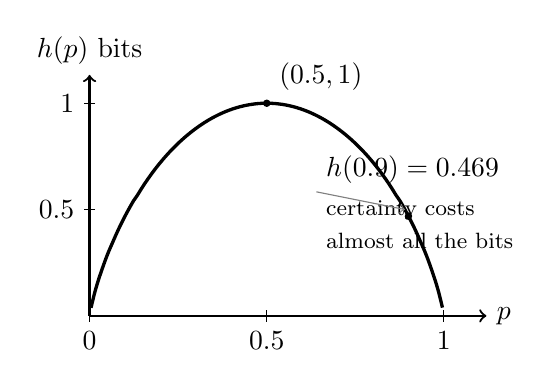
\begin{tikzpicture}[scale=0.9]
\draw[->, thick] (0,0) -- (5.6,0) node[right] {$p$};
\draw[->, thick] (0,0) -- (0,3.4) node[above] {$h(p)$ bits};
\foreach \x/\xl in {0/0, 2.5/0.5, 5/1}
  \draw (\x,0.08) -- (\x,-0.08) node[below] {\xl};
\foreach \y/\yl in {1.5/0.5, 3/1}
  \draw (0.08,\y) -- (-0.08,\y) node[left] {\yl};
% h(p) = -p log2 p - (1-p) log2(1-p), sampled
\draw[very thick, domain=0.02:4.98, smooth, samples=100]
  plot (\x, {3*(-(\x/5)*ln(\x/5)/ln(2) - (1-\x/5)*ln(1-\x/5)/ln(2))});
\fill (2.5,3) circle (1.5pt) node[above right=1pt] {$(0.5, 1)$};
\fill (4.5,{3*0.469}) circle (1.5pt);
\node[align=left, anchor=west] at (3.2,1.6) {$h(0.9)=0.469$\\[2pt]
  \footnotesize certainty costs\\ \footnotesize almost all the bits};
\draw[->, gray] (3.2,1.75) -- (4.45,1.5);
\end{tikzpicture}

\caption{The Bernoulli entropy curve $h(p)$. Notice: maximum at
$p=\tfrac12$ (1 bit), and how steeply information collapses as the
coin gets predictable --- $p=0.9$ keeps only $0.47$ bits. Regenerate:
\texttt{figures/ch15\_bernoulli.tex}.}\label{fig:bernh}
\end{figure}

\begin{figure}[htbp]\centering
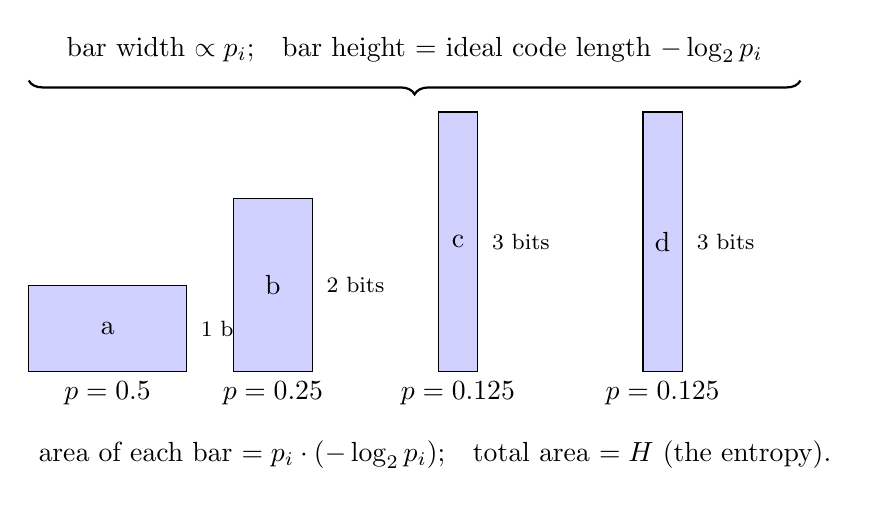
\begin{tikzpicture}[scale=1.0]
% colah-style: each symbol's bar shows -log2 p as its ideal code length.
% 4 symbols: p = 1/2, 1/4, 1/8, 1/8  -> lengths 1, 2, 3, 3
\foreach \i/\p/\len/\name in {0/0.5/1/a, 1/0.25/2/b, 2/0.125/3/c, 3/0.125/3/d}{
  \pgfmathsetmacro{\w}{4*\p}
  \draw[fill=blue!18] (\i*2.6,0) rectangle ({\i*2.6+\w},{1.1*\len});
  \node at ({\i*2.6+\w/2},{0.55*\len}) {\name};
  \node[below] at ({\i*2.6+\w/2},0) {$p=\p$};
  \node[right, font=\footnotesize] at ({\i*2.6+\w+0.06},{0.55*\len})
    {\len\ifnum\len>1 ~bits\else ~bit\fi};
}
\draw[decorate, decoration={brace, amplitude=5pt}, thick] (9.8,3.7) -- (0,3.7);
\node[align=center, above] at (4.9,3.8) {bar width $\propto p_i$;\quad
  bar height $=$ ideal code length $-\log_2 p_i$};
\node[align=left, anchor=north west] at (0,-0.75) {area of each bar
  $=p_i\cdot(-\log_2 p_i)$;\quad total area $=H$ (the entropy).};
\end{tikzpicture}

\caption{Ideal code lengths for $p=(\tfrac12,\tfrac14,\tfrac18,
\tfrac18)$: bar width is probability, bar height is $-\log_2 p$. Total
area is the entropy --- the picture behind the entropy-as-length
bound. Regenerate: \texttt{figures/ch15\_codeword.tex}.}
\label{fig:codeword}
\end{figure}

\begin{figure}[htbp]\centering
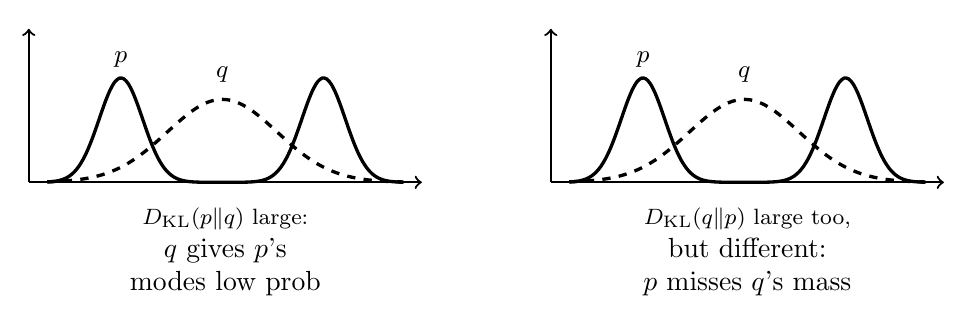
\begin{tikzpicture}[scale=0.78]
% two small multiples: target p bimodal; q single central bump
\foreach \cx/\captext in {0/{$D_{\mathrm{KL}}(p\|q)$ large:\\ $q$ gives $p$'s\\ modes low prob}, 8.5/{$D_{\mathrm{KL}}(q\|p)$ large too,\\ but different:\\ $p$ misses $q$'s mass}}{
  \begin{scope}[xshift=\cx cm]
    \draw[->, thick] (0,0) -- (6.4,0);
    \draw[->, thick] (0,0) -- (0,2.5);
    % p: bimodal
    \draw[very thick, domain=0.3:6.1, smooth, samples=80]
      plot (\x, {1.7*exp(-((\x-1.5)^2)/0.25) + 1.7*exp(-((\x-4.8)^2)/0.25)});
    \node[font=\small] at (1.5,2.0) {$p$};
    % q: single center bump
    \draw[very thick, dashed, domain=0.3:6.1, smooth, samples=80]
      plot (\x, {1.35*exp(-((\x-3.15)^2)/1.6)});
    \node[font=\small] at (3.15,1.75) {$q$};
    \node[align=center, below] at (3.2,-0.25) {\footnotesize\captext};
  \end{scope}
}
\end{tikzpicture}

\caption{Forward vs.\ reverse KL on a bimodal target $p$ and a
single-bump model $q$. Notice: each direction penalizes a different
kind of mismatch --- neither ``covers'' the other. Regenerate:
\texttt{figures/ch15\_kldirections.tex}.}\label{fig:kldir}
\end{figure}

\begin{figure}[htbp]\centering
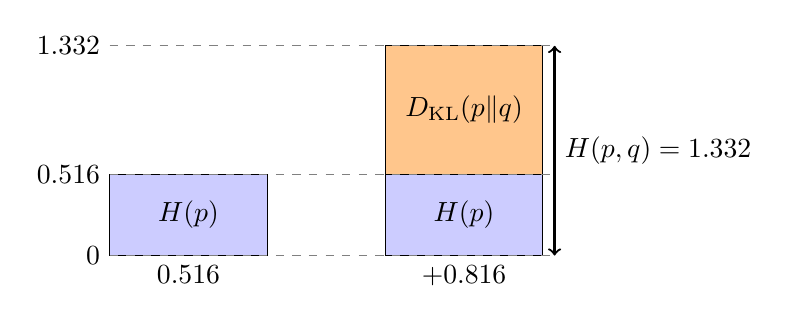
\begin{tikzpicture}[scale=1.0]
% stacked bars: H(p,q) = H(p) + KL(p||q)   (numbers from ch15_info.py)
% bar 1: H(p)
\draw[fill=blue!20] (0,0) rectangle (2,1.032);
\node at (1,0.52) {$H(p)$};
\node[below] at (1,0) {$0.516$};
% bar 2: H(p) + KL stacked = H(p,q)
\draw[fill=blue!20] (3.5,0) rectangle (5.5,1.032);
\draw[fill=orange!45] (3.5,1.032) rectangle (5.5,2.664);
\node at (4.5,0.52) {$H(p)$};
\node at (4.5,1.85) {$D_{\mathrm{KL}}(p\|q)$};
\node[below] at (4.5,0) {$+0.816$};
\draw[<->, thick] (5.65,0) -- (5.65,2.664) node[midway, right] {$H(p,q)=1.332$};
\foreach \y/\yl in {0/0, 1.032/{0.516}, 2.664/{1.332}}{
  \draw[gray, dashed] (0,\y) -- (5.6,\y);
  \node[left] at (0,\y) {\yl};
}
\end{tikzpicture}

\caption{$H(p,q)=H(p)+D_{\mathrm{KL}}(p\|q)$ on the listing's real
numbers ($0.516+0.816=1.332$ bits). Notice: the KL term is the only
part a model can shrink. Regenerate:
\texttt{figures/ch15\_cedecomp.tex}.}\label{fig:cedecomp}
\end{figure}

\begin{figure}[htbp]\centering
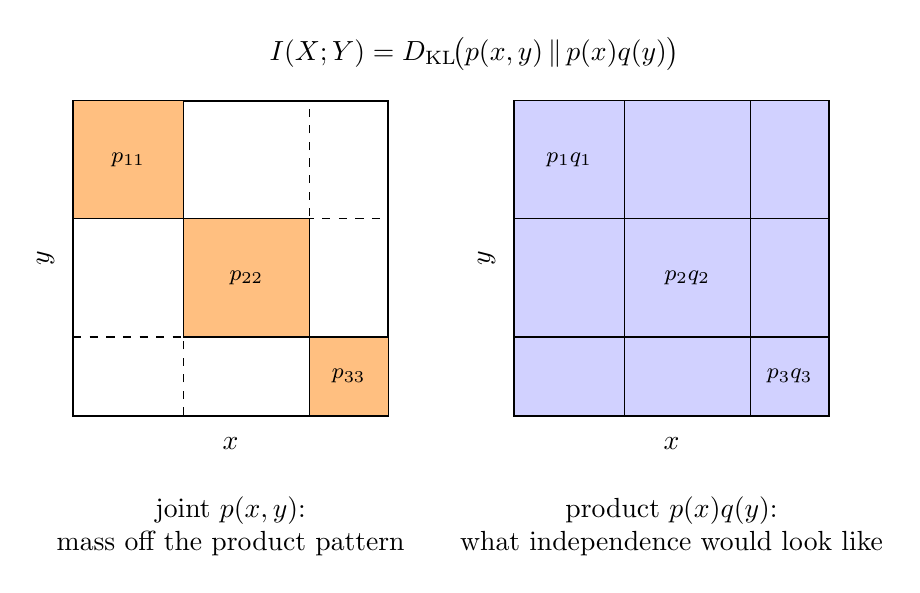
\begin{tikzpicture}[scale=1.0]
% unit square = p(x,y) mass; independent bands vs correlated mass
\draw[thick] (0,0) rectangle (4,4);
\draw[dashed] (0,1) -- (4,1); \draw[dashed] (0,2.5) -- (4,2.5);
\draw[dashed] (1.4,0) -- (1.4,4); \draw[dashed] (3,0) -- (3,4);
\node[rotate=90] at (-0.35,2) {$y$};
\node at (2,-0.35) {$x$};
% correlated mass concentrated near diagonal blocks
\draw[fill=orange!50] (0,2.5) rectangle (1.4,4);
\draw[fill=orange!50] (1.4,1) rectangle (3,2.5);
\draw[fill=orange!50] (3,0) rectangle (4,1);
\node[font=\footnotesize] at (0.7,3.25) {$p_{11}$};
\node[font=\footnotesize] at (2.2,1.75) {$p_{22}$};
\node[font=\footnotesize] at (3.5,0.5) {$p_{33}$};
\begin{scope}[xshift=5.6cm]
  \draw[thick] (0,0) rectangle (4,4);
  \draw[dashed] (0,1) -- (4,1); \draw[dashed] (0,2.5) -- (4,2.5);
  \draw[dashed] (1.4,0) -- (1.4,4); \draw[dashed] (3,0) -- (3,4);
  \foreach \i/\a/\b in {0/0/1.4, 1/1.4/3, 2/3/4}{
    \foreach \j/\c/\d in {0/0/1, 1/1/2.5, 2/2.5/4}{
      \draw[fill=blue!18] (\a,\c) rectangle (\b,\d);}}
  \node[font=\footnotesize] at (0.7,3.25) {$p_1 q_1$};
  \node[font=\footnotesize] at (2.2,1.75) {$p_2 q_2$};
  \node[font=\footnotesize] at (3.5,0.5) {$p_3 q_3$};
  \node[rotate=90] at (-0.35,2) {$y$};
  \node at (2,-0.35) {$x$};
\end{scope}
\node[below, align=center] at (2,-0.9) {joint $p(x,y)$:\\ mass off the product pattern};
\node[below, align=center] at (7.6,-0.9) {product $p(x)q(y)$:\\ what independence would look like};
\node[align=left] at (5.1,4.6) {$\displaystyle I(X;Y)=
  D_{\mathrm{KL}}\!\big(p(x,y)\,\|\,p(x)q(y)\big)$};
\end{tikzpicture}

\caption{Mutual information compares the joint (left, mass piled near
the diagonal) with the product of marginals (right, what independence
would predict). Notice: $I(X;Y)$ is the KL between the two pictures.
Regenerate: \texttt{figures/ch15\_mi.tex}.}\label{fig:midiagram}
\end{figure}

\begin{figure}[htbp]\centering
\begin{tikzpicture}[scale=0.9]
\draw[->, thick] (0,0) -- (6.4,0) node[right] {$\sigma$};
\draw[<->, thick] (0,-1.4) -- (0,3) node[above] {$h(X)$ nats};
% h = 0.5 ln(2 pi e s^2) = ln(s) + 1.419 ; zero at s ~ 0.242
% scale: x = s*2.4 (s 0..2.5), y = (ln s + 1.419)*1.3
\draw[very thick, domain=0.24:6.2, smooth, samples=80]
  plot (\x, {1.3*(ln(\x/2.4) + 1.419)});
\fill ({2.4*0.242},0) circle (1.4pt) node[below right] {$\sigma\approx0.24$: $h=0$};
\foreach \x/\xl in {2.4/1, 4.8/2}
  \draw (\x,0.06) -- (\x,-0.06) node[below] {\xl};
\draw[gray, dashed] (0,0) -- (6.2,0);
\node[align=left, anchor=west] at (3.4,-1.0) {$h=\tfrac12\ln(2\pi e\sigma^2)$\\
  differential entropy can be\\ negative --- it is not\\ information, just spread.};
\end{tikzpicture}

\caption{Gaussian differential entropy vs.\ $\sigma$. Notice: $h$
crosses zero near $\sigma\approx0.24$ and goes negative ---
differential entropy measures spread, not information. Regenerate:
\texttt{figures/ch15\_gaussent.tex}.}\label{fig:gaussent}
\end{figure}
